\apendice{Especificación de diseño}

\section{Introducción}
En este capítulo veremos  todo lo relacionado con el diseño de la herramienta.
\section{Diseño de datos}
El diseño tanto visual como de los datos, se decidió antes de empezar a realizar el proyecto. Se basa en:
\begin{itemize}
\item Diseño visual organizado en Frames y ordenado por paquetes (Packs de Tkinter \cite{pack}). Los packs permiten subdividir cada pantalla en pequeñas proporciones y estas en subproporciones, así sucesivamente. .
\item Alimentos tratados según el estándar de medida nutricional, por cada 100 gramos \cite{estandarNutri}.
\item Bases de datos en archivos ".xlsx".
\item Manejo interno de los datos a través de DataFrames.
\end{itemize}
\section{Diseño procedimental}
\subsection{Introducción}
A continuación, se definirá la forma de funcionamiento de las acciones realizadas por la aplicación a pro de la utilidad del proyecto. Todos los diseños han sido realizados con la herramienta "Draw.io" \cite{herramientoUML}.
\subsubsection{Alta o modificación de usuarios}
El alta y modificación de usuarios parten de la misma estructura del funcionamiento, variando simplemente en un pequeño paso que será indicado en su momento. Antes de comenzar con el análisis detallado se mostrará a grandes rasgos la estructura principal externa de este proceso:\\
\begin{enumerate}
\item El usuario rellena sus datos y valida.
\item El programa comprueba que todo es correcto. Si es así lo añade, sino lanza un error.
\end{enumerate}
Así es como funcionaría el algoritmo paso a paso:
\begin{itemize}
\item Inicio.
\item Solicitar los datos a rellenar.
\item Enviar dichos campos al módulo de administración (AdminBase) para su comprobación.
\item Si algún dato es erróneo se muestra el mensaje de error, sino sigue su ejecución.
\item Si es alta de usuario añade información del nuevo usuario a la base de datos.
\item Si es modificación de datos busca al usuario existente y remplaza.
\end{itemize}
Se muestra el diagrama de interacción de los diferentes objetos.
\imagen{UMLRegistro}{Diagrama UML sobre la interacción en el registro o modificación de un usuario}
\subsection{Elegir Alimento}
En este caso, es algo más complicado que lo anterior, pues hay varias vertientes. Es posible refrescar hasta encontrar el alimento buscado, y cuando es seleccionado se actualizan el resto de Frames.
\begin{itemize}
\item El usuario refresca la página hasta encontrar su elección. 
\item El usuario elige y se almacena en su registro diario esa elección.
\item El programa actualiza automáticamente el resto de Frames.
\end{itemize}
Se detalla cada paso del procedimiento explicado anteriormente:
\begin{enumerate}
\item El usuario se incorpora al Frame de selección.
\item El usuario decide si escoger una opción o buscar otra.
\begin{itemize}
\item Si escoge una opción se almacenan los datos, y se actualizan el resto de posibles elecciones.
\item Si refresca la página en busca de otros alimentos, se suma los valores de uso a esas comidas y se recomiendan unas nuevas.
\end{itemize}
\item Sigue el programa hasta que el usuario salga de la ventana, y se mantienen las elecciones registradas.
\end{enumerate}
Diagrama UML de la interacción del programa en la selección. \\
\imagen{UMLSeleccion}{Diagrama UML que muestra la interacción entre frames y funciones durante la selección}
\pagebreak

Seguidamente se visualiza un diagrama de flujo  similar al anterior, pero sobre el refrescar de las opciones y con otro método diferente a UML:
\begin{figure}[h]
\centering
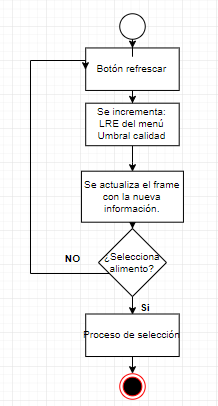
\includegraphics[scale=1]{DiagramaFlujoRefrescar}
\caption{Diagrama de flujo de la acción de refrescar opciones de menú}
\label{figura:refrescar}
\end{figure}
\pagebreak
\subsection{Carga y almacenamiento bases de datos}
Teniendo en cuenta la similitud entre el funcionamiento de la carga y almacenamiento de datos de las diferentes colecciones, se pasa a describir un modelo general que engloba a todos ellos:
\begin{itemize}
\item El usuario inicia la aplicación.
\item Se cargan automáticamente los datos.
\begin{itemize}
\item Se abren los diferentes Excel que simulan la base de datos.
\item Se traducen a DataFrame con el nombre de columna como el nombre del objeto de la colección.
\end{itemize}
\item Se tratan los vectores por separado evitando romper la consistencia de la base de datos.
\item Cuando el usuario guarda los datos, se sustituye la base de datos por el DataFrame actual.
\end{itemize}
\imagen{UMLBD}{Diagrama UML de la interacción básica del programa con la base de datos.}
\subsection{Estructura general del programa}
Diagrama del funcionamiento e interacción de la estructura del programa completo.
\begin{itemize}
\item Se crea la ventana de Inicio.
\item El usuario inicia sesión o se registra.
\begin{itemize}
\item Registro: Añade toda la información y si es correcta se le añade a la base de datos, sino se le muestra un mensaje de error.
\item Inicio de sesión:
\begin{itemize}
\item Se le muestra la pantalla principal con tres vertientes.
\begin{itemize}
\item Información de usuario.
\item Dieta.
\item Historial.
\end{itemize}
\item El usuario hace un correcto uso de la aplicación.
\item Se guardan los diferentes cambios a voluntad del usuario.
\item Se cierra la aplicación.
\end{itemize}
\end{itemize}
\end{itemize}
A continuación se mostrará un diagrama UML básico de la interacción del usuario con el programa, en caso de haber iniciado sesión.
\imagen{UMLGeneral}{Diagrama UML general del programa, una vez se ha iniciado sesión.}
\section{Diseño arquitectónico}
El diseño arquitectónico lo separaremos en dos partes principales para mejorar su entendimiento. La idea principal es separar la arquitectura visual entre Frames, el cual contiene un sistema de herencia en la navegabilidad, y la estructura modular con las diferentes funciones internas.
\pagebreak
\subsection{Arquitectura visual}
\begin{figure}[h]
\centering
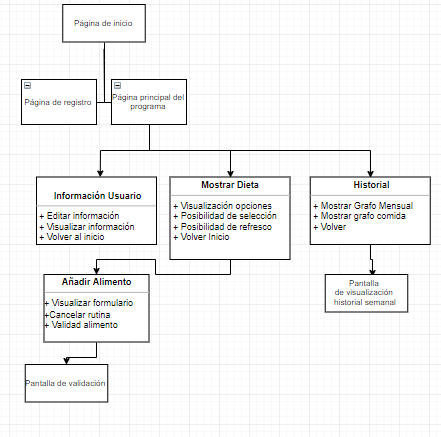
\includegraphics[scale=1]{ArquitecturaVisual}
\caption{Imagen de la consiguiente arquitectura visual para la correcta navegación}
\label{figura:arquitecturaVisual}
\end{figure}
\subsection{Arquitectura Modular}
Para esta arquitectura se tendrá en cuenta dos diagramas principales. Dado la complejidad del Main, se realizará un diagrama general y otro particular para el interior del Main. Debido al tamaño de cada módulo y para una visualización más clara, primero se visualizará el diagrama de conexiones y luego el diagrama de clases de cada módulo.\\
\subsubsection{Diagrama de módulos}
Antes de ver la imagen de relaciones entre módulos, aclarar que cuando la flecha sale de un módulo al siguiente es que ese módulo hace uso del otro, pero no viceversa (excepto en flechas bidireccionales).
\imagen{DiagramaRelaciones}{Diagrama de las relaciones generales entre los distintos módulos.}
\pagebreak
\textbf{Vista}\\
\begin{figure}[h]
\centering
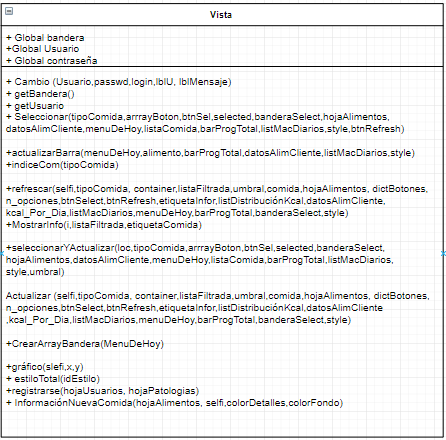
\includegraphics[scale=1]{DiagramaVista}
\caption{Diagrama de clases del módulo/clase vista.}
\label{figura:DiagramaVista}
\end{figure}
\pagebreak

\textbf{AdminBase}\\
\imagen{DiagramaAdmin}{Diagrama de clases del módulo/clase AdminBase.}
\textbf{CalculosDieta}\\
\imagen{DiagramaCalculos}{Diagrama de clases del módulo/clase CalculosDieta.}
\pagebreak
\subsubsection{Diagrama Interno del Main}
Debido a la mecánica de la librería Tkinter, fue necesario crear cada Frame dentro de la misma clase, para que generara el flujo que principalmente se usa durante el programa. Por ello, hay una jerarquía propia de clases dentro del propio Main.
\imagen{DiagramaMain}{Diagrama interno del Main}